%% (Master) Thesis template
% Template version used: v1.4
%
% Largely adapted from Adrian Nievergelt's template for the ADPS
% (lecture notes) project.


%% We use the memoir class because it offers a many easy to use features.
\documentclass[11pt,a4paper]{memoir}

%% CUSTOM Marc: Decrease Margins
\setlrmarginsandblock{3cm}{3cm}{*}
\setulmarginsandblock{3cm}{*}{1}
\checkandfixthelayout 

%% Packages
%% ========

%% LaTeX Font encoding -- DO NOT CHANGE
\usepackage[OT1]{fontenc}

%% Babel provides support for languages.  'english' uses British
%% English hyphenation and text snippets like "Figure" and
%% "Theorem". Use the option 'ngerman' if your document is in German.
%% Use 'american' for American English.  Note that if you change this,
%% the next LaTeX run may show spurious errors.  Simply run it again.
%% If they persist, remove the .aux file and try again.
\usepackage[english]{babel}

%% Input encoding 'utf8'. In some cases you might need 'utf8x' for
%% extra symbols. Not all editors, especially on Windows, are UTF-8
%% capable, so you may want to use 'latin1' instead.
\usepackage[utf8]{inputenc}

%% This changes default fonts for both text and math mode to use Herman Zapfs
%% excellent Palatino font.  Do not change this.
\usepackage[sc]{mathpazo}

%% The AMS-LaTeX extensions for mathematical typesetting.  Do not
%% remove.
\usepackage{amsmath,amssymb,amsfonts,mathrsfs}

%% NTheorem is a reimplementation of the AMS Theorem package. This
%% will allow us to typeset theorems like examples, proofs and
%% similar.  Do not remove.
%% NOTE: Must be loaded AFTER amsmath, or the \qed placement will
%% break
\usepackage[amsmath,thmmarks]{ntheorem}

%% LaTeX' own graphics handling
\usepackage{graphicx}


%% This allows you to add .pdf files. It is used to add the
%% declaration of originality.
\usepackage{pdfpages}

\usepackage{realboxes}
\usepackage{listings}
\lstdefinelanguage{none}{
  identifierstyle=
}
\definecolor{backcolor}{rgb}{0.95,0.95,0.92}
\lstdefinestyle{mystyle}{
    backgroundcolor=\color{backcolor}
}
\newcommand{\inline}[1]{\Colorbox{backcolor}{\lstinline[language=C]{#1}}}



%% Our layout configuration.  DO NOT CHANGE.
\input{layoutsetup}

%% Theorem environments.  You will have to adapt this for a German
%% thesis.
\input{theoremsetup}


%% Make document internal hyperlinks wherever possible. (TOC, references)
%% This MUST be loaded after varioref, which is loaded in 'extrapackages'
%% above.  We just load it last to be safe.
\usepackage[linkcolor=black,colorlinks=true,citecolor=black,filecolor=black]{hyperref}

% ######## CUSTOM package load before cleverref ########
\RequirePackage{silence}
\WarningFilter{latexfont}{Font shape `}
\WarningFilter{latexfont}{Size substitutions}

\usepackage{stmaryrd}
\usepackage[advantage,adversary,sets,ff,primitives,events,keys,notions]{cryptocode}
\usepackage{siunitx}

\usepackage{multirow}
\usepackage{adjustbox}
\usepackage{xspace}
% ######## END CUSTOM package load ########

%% This allows you to use "\cref{sec:your-section}" instead of writing out 
%% "Section~\ref{sec:your-section}", also works for tables, figures, etc.
%% Use \Cref at the beginning of a sentence and \cref elsewhere.
%% Must be loaded after hyperref.
\usepackage[capitalise]{cleveref}


%% Document information
%% ====================

\title{Implementing and Evaluating Quantum-Safe Fully Encrypted Protocols}
\author{Marc Himmelberger}
\thesistype{Master's Thesis}
\advisors{Advisors: Prof.~Kenneth G. Paterson, Dr.~Felix Günther (IBM Research - Zürich), Shannon Veitch}
\department{Applied Cryptography Group\\Institute of Information Security\\Department of Computer Science}
\date{June 20, 2025}

% ######## CUSTOM style code ########
\lstdefinestyle{myStyle}{
    breaklines=true,
    frame=leftline,
    numbers=left,
    backgroundcolor=\color{gray!10!white},
}
\lstset{style=myStyle}

\newcolumntype{L}[1]{>{\raggedright\arraybackslash}p{#1}}
\newcolumntype{R}[1]{>{\raggedleft\arraybackslash}p{#1}}
\newcommand{\getsr}{\xleftarrow{\smash{\raisebox{-1.75pt}{$\scriptscriptstyle\$$}}}}
\newcommand{\tor}{\xrightarrow{\smash{\raisebox{-1.75pt}{$\scriptscriptstyle\$$}}}}
\newcommand{\ul}[1]{\underline{\smash{#1}}}  % tight underline
\newcommand{\KEM}{\ensuremath{\mathsf{KEM}}}
\newcommand{\OKEM}{\ensuremath{\mathsf{OKEM}}}
\newcommand{\pkcoll}[1]{\pcnotionstyle{pkcoll}_{#1}}
\newcommand{\obfpklen}{{\mathsf{pl}_\OKEM}}
\newcommand{\obfctxtlen}{{\mathsf{cl}_\OKEM}}
\newcommand{\pklen}{{\mathsf{pl}_\KEM}}
\newcommand{\ctxtlen}{{\mathsf{cl}_\KEM}}
\newcommand{\pkobf}{\hat{\pk}}

\newcommand{\simulbin}{\mathcal{S}_\$}
\newcommand{\simulunif}{\mathcal{S}_\mathcal{C}}

\newcommand{\feo}{\textsf{\textnormal{FEO}}}

\newcommand{\obfsfour}{\textsf{obfs4}}
\newcommand{\pqobfs}{\textsf{pq-obfs}}
\newcommand{\drivel}{\textsf{drivel}}

\newcommand{\gopkgref}[2]{\href{https://pkg.go.dev/#1@#2}{#1} #2}

\pcfixcleveref

% Define aliases
\renewcommand{\pcadvantagename}{\mathsf{Adv}}
\renewcommand{\pcadvantagesuperstyle}[1]{#1}
\renewcommand{\pcadvantagesubstyle}[1]{#1}

% Set up style for algorithms
\definecolor{lngray}{gray}{0.5} % gray line numbers
\renewcommand{\pclnspace}{0.5em} % spacing of numbering
\renewcommand{\pclnrspace}{0em}
\renewcommand{\pclnstyle}[1]{\text{\scriptsize\color{lngray} \num[minimum-integer-digits=2]{#1}}} % zero-pad
\renewcommand{\pclnseparator}{} % no separator
\makeatletter % put comments at the end of lines, could not do it just with hfill & fiends so I dug into internals :P
\newcommand{\lncomment}[1]{ \@pc@modeend& \mbox{\pccomment{}\hspace{-0.75em} \ensuremath{#1}} \\  }
\newcommand{\titlecomment}[1]{ \hfill \mbox{\pccomment{}\hspace{-0.75em} \ensuremath{#1}}}
\makeatother
% Refine cryptocode styles and add more notions
\renewcommand{\pcnotionstyle}[1]{\ensuremath{\mathsf{#1}}}
\renewcommand{\kgen}{\pcalgostyle{KeyGen}}

\providecommand{\encaps}{\pcalgostyle{Encaps}}
\providecommand{\decaps}{\pcalgostyle{Decaps}}
\providecommand{\decapsoracle}{\mathcal{O}_{\decaps}}
\providecommand{\filterpk}{\pcalgostyle{FilterPk}}
\providecommand{\encodectxt}{\pcalgostyle{EncodeCtxt}}
\providecommand{\decodectxt}{\pcalgostyle{DecodeCtxt}}
\providecommand{\sprcca}{\pcnotionstyle{SPR\pcmathhyphen{}CCA}}
\providecommand{\sprcpa}{\pcnotionstyle{SPR\pcmathhyphen{}CPA}}

\providecommand{\sObfKE}{\pcnotionstyle{sObfKE}}
\providecommand{\swapprf}{\pcnotionstyle{swap\pcmathhyphen{}PRF}}
\providecommand{\indonecca}{\pcnotionstyle{IND\pcmathhyphen{}1CCA}}

\providecommand{\firstkeygensuccess}{\pcnotionstyle{1kgensucc}}
\providecommand{\firstencapssuccess}{\pcnotionstyle{1encsucc}}

\providecommand{\pkunif}{\pcnotionstyle{pk\pcmathhyphen{}unif}}
\providecommand{\ctxtunif}{\pcnotionstyle{ctxt\pcmathhyphen{}unif}}

\providecommand{\prkey}{\pcnotionstyle{PR\pcmathhyphen{}Key}}
\providecommand{\mdsd}{\pcnotionstyle{mDSD}}
\providecommand{\skdsd}{\pcnotionstyle{skDSD}}


\providecommand{\twodqcsd}{\pcnotionstyle{2\pcmathhyphen{}DQCSD}}
\providecommand{\threedqcsd}{\pcnotionstyle{3\pcmathhyphen{}DQCSD}}

\providecommand{\sObf}{\pcnotionstyle{sObf}}

% ######## Start macros.tex

\definecolor{RoyalBlue}{RGB}{65,105,225}

% ClientAction and ServerAction
% Print a command executed by the client/server
% main argument: the text, optional argument: tikz modifier
\newcommand{\ClientAction}[2][]{
	\node[right,#1] at (\ClientX, \Y) {#2};
}
\newcommand{\ServerAction}[2][]{
	\node[left,#1] at (\ServerX, \Y) {#2};
}
\newcommand{\ServerActionLeft}[2][]{
	\ServerAction[text width=\ServerLeftTextwidth,align=left,#1]{#2}
}
\newcommand{\SharedAction}[2][]{
	\node[#1] at ($1/2*(\ClientX, \Y)+1/2*(\ServerX, \Y)$) {#2};
}

% ClientToServer and ServerToClient
% Draws a message flow from client-to-server or server-to-client, with text above and below
% 1st argument (optional): line type, default ->
% 2nd argument: text above
% 3rd argument: text below
% Example: \ClientToServer{$Y$}{}
% Example: \ClientToServer[<->,double]{$Y$}{over an encrypted channel}
\newcommand{\ClientToServer}[3][->]{
	\NextLine[0.5]
	\draw[#1] (\ArrowLeft,\Y) -- node[above] {#2} node[below] {#3} (\ArrowRight,\Y) ;
	% \NextLine[0.5]
}
\newcommand{\ServerToClient}[3][->]{
	\NextLine[0.5]
	\draw[#1] (\ArrowRight,\Y) -- node[above] {#2} node[below] {#3} (\ArrowLeft,\Y) ;
	% \NextLine[0.5]
}
% Draws a horizontal line across the entire page to denote the start and end of protocol phases
% 1st argument (optional): line type, default "dotted"
% 2nd argument: text above
% 3rd argument: text below
\newcommand{\PhaseBreak}[3][dotted]{
	\NextLine[0.5]
	\draw[#1] (\ClientX,\Y) -- node[above] {#2} node[below] {#3} (\ServerX,\Y) ;
	% \NextLine[0.5]
}

% Spacing factor for NextLines
\def\NextLineSpacing{0.45}

% NextLine
% 1st argument (optional): amount of spacing to increment by, default 1.0
% Example: \NextLine
% Example: \NextLine[1.5]
\newcommand{\NextLine}[1][1.0]{
	\pgfmathparse{\Y-\NextLineSpacing*#1}
	\edef\Y{\pgfmathresult}
}


\newcommand{\highlightbox}[2][RoyalBlue!20]{\adjustbox{cframe=#1, bgcolor=#1}{\strut #2}}

\providecommand{\nodeid}{\ensuremath{\mathsf{NodeID}}}
\providecommand{\nodeidlen}{\ensuremath{\mathsf{nl}}}
\providecommand{\pstate}{\ensuremath{\mathsf{st}}}
\providecommand{\macregister}{\ensuremath{\mathcal{S}_\mathsf{MAC}}}
\providecommand{\cpaddist}{\ensuremath{\mathcal{D}_\mathsf{pad}_C}}
\providecommand{\cpaddist}{\ensuremath{\mathcal{D}_\mathsf{pad}_S}}

\newcommand{\funPRF}{\ensuremath{\pcalgostyle{F}_1}\xspace}
\newcommand{\funPRFoutlen}{\ensuremath{\mathsf{fl}_1}}
\newcommand{\funComb}{\ensuremath{\pcalgostyle{F}_2}\xspace}
\newcommand{\funComboutlen}{\ensuremath{\mathsf{fl}_2}}

\newcommand{\symmenc}{\pcalgostyle{SE}}
\newcommand{\funEnc}{\pcalgostyle{\symmenc.Enc}}
\newcommand{\funDec}{\pcalgostyle{\symmenc.Dec}}

\newcommand{\keylen}{\ensuremath{\mathsf{kl}}}
\newcommand{\textlit}[1]{\ensuremath{\text{``\texttt{#1}''}}}

\providecommand{\conc}{\|}
\crefname{conjecture}{Conjecture}{Conjectures}

% ######## END CUSTOM style code ########

\begin{document}

\frontmatter

%% Title page is autogenerated from document information above.  DO
%% NOT CHANGE.
\begin{titlingpage}
  \calccentering{\unitlength}
  \begin{adjustwidth*}{\unitlength-24pt}{-\unitlength-24pt}
    \maketitle
  \end{adjustwidth*}
\end{titlingpage}

%% The abstract of your thesis.  Edit the file as needed.
\begin{abstract}
The Tor network enables anonymous communication by routing traffic through volunteer-operated relays, but access to the network is often restricted through censorship that targets identifiable protocol patterns.
In order to counteract such restrictions, protocols must resist fingerprinting, for example, by obfuscating their traffic to appear like random bytes on the wire.

In this thesis, we adapt the Tor Project's lyrebird implementation to include the obfuscated key exchange protocol \drivel{}, which extends the \obfsfour{} protocol with post-quantum security and stronger obfuscation.
We analyze the Classic-McEliece and HQC key exchange mechanisms, defining mappings from ciphertexts to random byte strings required for their deployment in \drivel{}. These schemes are then integrated with our implementation, in addition to the previously examined ML-KEM and FrodoKEM schemes.
Finally, we empirically evaluate our implementation using benchmarks and deployments under laboratory conditions and suggest concrete changes to \drivel{} to increase performance and reduce identifiable traffic patterns in the handshake.
\end{abstract}

\clearpage
\section*{Acknowledgement}
I would like to extend my thanks first to my supervisors Shannon Veitch, Dr.~Felix Günther and Prof.~Dr.~Kenny Paterson for guiding me towards this engaging topic and giving me the opportunity to apply my skills for both theoretical analyses as well as a practical implementation. Their ideas and feedback in every discussion served to improve my thesis tremendously and I am grateful for the chance to contribute to such a relevant topic.

In addition, I want to thank Dr.~Keita Xagawa for his time and insights, which helped me better understand prior research in the space of anonymity of quantum-safe KEMs.

Finally, I thank my friends, colleagues, family, my fiancée, and our cat --- for keeping me motivated, for listening to many overly-technical explanations of my thesis, and for supporting me in more ways than I can count throughout the entirety of my studies.

%% TOC with the proper setup, do not change.
\cleartorecto
\tableofcontents
\mainmatter

%% Your real content!
\sloppy
\chapter{Introduction}\label{ch:intorduction}

Reusing proposal document for starting sections.

Differentiate obfs4 against VMess or Shadowsocks.

\section{Our contributions} \label{sec:contributions}

\section{Related Work} \label{sec:related-work}

\chapter{Preliminaries}\label{ch:preliminaries}

\section{\texorpdfstring{Review of Günther, Stebila, and Veitch \cite{CCS:GunSteVei24}}{Review of Günther, Stebila, and Veitch}} \label{sec:review-gsv24}

Günther et al. first described a framework for proveable security of obfuscated key exchange, extending efforts by Fenske and Johnson \cite{CCS:FenJoh24}, whose work focused on the data transfer phase of fully encrypted protocols.

For convenience, we reproduce the central definitions, that this thesis interfaces with, here.

WATCH OUT: USE ABSOLUTE VALUE IN ADVANTAGES, EASES GAME HOPPING

\begin{definition}\label{def:keygen-then-encode}
    2.2 keygen-then-encode oKeyGen construction
\end{definition}

\begin{definition}\label{def:first-keygen-success}
    2.3 first keygen success prob.
\end{definition}

\begin{definition}\label{def:pk-uniformity}
    2.4 public key uniformity
\end{definition}

TODO: Note that even though 2.3 and 2.4 are defined for obfuscated key generation only, the definitions are compatible with OKEM.

\begin{definition}\label{def:okem}
    2.5 OKEM
\end{definition}

\begin{definition}\label{def:okem-correctness}
    2.6 OKEM correctness
\end{definition}

\begin{definition}\label{def:pk-collisions}
    2.7 public key collisions
\end{definition}

\begin{definition}\label{def:keygen-encap-then-encode}
    2.8 Keygen/Encap-then-encode OKEM construction
\end{definition}

\begin{definition}\label{def:first-encap-success}
    2.9 First encap success prob.
\end{definition}

\begin{definition}\label{def:ctxt-uniformity}
    2.10 ciphertext uniformity
\end{definition}

\begin{definition}\label{def:ind-spr-cca}
    2.11 IND-CCA, SPR-CCA for a KEM (note that simulator doesn't matter so long as proof goes through)
\end{definition}

\begin{theorem}\label{thm:s-obfuscated-keyex-security}
    7.1 For full protocol security sObfKE; list all requirements
\end{theorem}
\chapter{Obfuscating NIST candidates}\label{ch:obfuscation}

In this section, we construct encodings for different post-quantum KEMs suitable for use in the pq-obfs protocol.

While such encodings have already been constructed for elliptic curve Diffie–Hellman \cite{CCS:BHKL13, tor-dev-udh, USENIX:WWGH11} as well as for ML-KEM \cite{CCS:GunSteVei24}, other KEMs are also being examined for future use.

TODO: Also cite 64, 62 from Obfuscated Key Exchange? Cite by name?

We take a selection of round 4 candidates of the NIST Post-Quantum Cryptography Standardization, as well as previous candidate schemes which we believe to be of interest.
For each scheme, we describe the generation of public keys and ciphertexts in the original scheme and examine their distributions. We then introduce encoding algorithms from the original public keys and ciphertexts to bitstrings and finally give concrete bounds for uniformity and encoding success rate.

We call all our encoding schemes TODO where TODO is the name of the corresponding KEM. \cref{tab:obfuscation-summary} summarizes the result of the later sections.

TODO: Show domain in table? Update references to convenience definitions earlier.

\begin{table}
    \centering
    \scriptsize\raggedright
    \begin{tabular}{@{} *{2}{L{0.125\textwidth-\tabcolsep}} | *{3}{L{0.25\textwidth-2\tabcolsep}} @{}}
        \textbf{KEM} & \textbf{Encoding} & \textbf{Obfuscation/Ciphertext uniformity} & \textbf{First-Keygen/Encap Success Probability} (\cref{def:first-keygen-success} and \ref{def:first-encap-success}) & \textbf{Output Size} (in bytes)\\ \hline
        Classic McEliece \cite{NISTPQC-R4:ClassicMcEliece22} & TODO &  &  & \\
         & - public keys & 0.01 & 0.2 & 0.3 \\
         & - ciphertexts & 0.01 & 0.2 & 0.3 \\
         &  &  &  & \\
    \end{tabular}
    \caption{Summary of KEMs, their corresponding encodings and the results of our analysis. The origins of analysis results are specified, and for output sizes, differences in bytes from original public key/ciphertext sizes are given. This table can be viewed as an extension of \cite[Table~2]{CCS:GunSteVei24}.}
    \label{tab:obfuscation-summary}
\end{table}

\section{Obfuscating Classic McEliece with TODO} \label{sec:obfuscating-classic-mceliece}

\paragraph{Original Generation and Distribution}
Classic McEliece \cite{NISTPQC-R4:ClassicMcEliece22} is a code-based KEM in round 4 of the NIST PQC standardization. We only consider the so-called "non-f" versions of the specified parameter sets which are interoperable with the f versions, and have simpler but slower key generation. TODO: OK? Keita also makes that assumption at some point.

In Classic McEliece, public keys are the rightmost column of a generator matrix in systematic form. Ciphertexts are the data bits corresponding to codewords with Hamming weight exactly $t$.

The generation of public keys occurs in a multi-step process starting from a 256-bit seed which is expanded using SHAKE256 into a secondary seed and raw values. If the raw values do not form a suitable systematic code, another attempt is started from the secondary seed, and so on.

For encapsulation, rejection-sampling is used to generate a uniformly random vector of Hamming weight $t$ which is then mapped from the space of $n$-bit vectors to $mt=n-k$ bits.

We define the same assumptions about computational hardness as in \cite[Definition~K.1]{EC:Xagawa22}. \cref{fig:classic-mceliece-assumptions} shows corresponding game-based definitions.
\begin{itemize}
    \item \textbf{PR-Key assumption:} It is computationally hard to distinguish real public keys from the rightmost columns of the systematic forms of uniformly random generator matrices (conditional on the systematic form existing). \\
    Consequently, no adversary $\adv$ could achieve high $ \advantage{\prkey}{}[(\adv)] $.
    \item \textbf{modified Decisional Syndrome Decoding assumption:} It computationally hard to distinguish real ciphertexts from uniformly random $(n-k)$-bit vectors. \\
    Consequently, no adversary $\adv$ could achieve high $ \advantage{\mdsd}{}[(\adv)] $.
\end{itemize}

\begin{figure}
    \begin{pchstack}[boxed, center, space=0.5em]

\begin{pcvstack}[space=0.05em]
\procedure[linenumbering]{$\textbf{GAME } \textsf{PR-Key}(\adv)$}{
    b \gets \bin \\
    (T_0,\sk) \gets \kgen() \\
    T_1 \gets \textsf{RandGen}() \\
    b' \gets \adv(T_b) \\
    \pcreturn \llbracket b' = b \rrbracket
}

\procedure[lnstart=5,linenumbering]{$\textbf{GAME } \textsf{mDSD}(\adv)$}{
    b \gets \bin \\
    \hat T \gets \textsf{RandGen}() \\
    e \gets \textsf{FixedWeight}() \\
    u_0 \gets \left[ I_{mt} \mid \hat T \right] \cdot e \\
    u_1 \gets U(\mathbb F_2^{mt}) \\
    b' \gets \adv(\hat T, u_b) \\
    \pcreturn \llbracket b' = b \rrbracket
}
\end{pcvstack}

\begin{pcvstack}[space=0.05em]
\procedure[lnstart=12,linenumbering]{$\textsf{RandGen}()$}{
    \hat T \gets \bot \\
    \pcwhile \hat T = \bot \pcdo \\
    \t  \hat H \gets U(\mathbb F_2^{mt \times n}) \\
    \t  \text{reduce } \hat H \text{ to systematic form } \left[ I_{mt} \mid \hat T \right] \\
    \label{ln:randgen-reject}
    \t  \text{if this fails } \hat T \gets \bot \\ 
    \pcendwhile \\
    \pcreturn \hat T
}

\procedure[lnstart=19,linenumbering]{$\textsf{RandGen}'()$}{
    \hat T \gets U(\mathbb F_2^{mt \times k}) \\ 
    \pcreturn \hat T
}
\end{pcvstack}

\end{pchstack}

    \caption{Indistinguishability games for Classic McEliece with $\kgen$ and \textsf{FixedWeight} as defined in \cite{NISTPQC-R4:ClassicMcEliece22}. These follow the definitions from \cite[Definition~K.1]{EC:Xagawa22}.}
    \label{fig:classic-mceliece-assumptions}
\end{figure}

\paragraph{Constructed Encoding}

\paragraph{Uniformity and Success Rate}


\section{Obfuscating ABC with XYZ} \label{sec:tbd}


\section{Classic McEliece as an Obfuscated KEM} \label{sec:obfuscating-classic-mceliece}

Throughout this \cref{sec:obfuscating-classic-mceliece}, we use the positive integer variables $m,n,t,k$ where $n < 2^m$ and $k=mt-n$ as defined in \cite{NISTPQC-R4:ClassicMcEliece22}. We work with matrices and vectors over $\mathbb F_2$ when examining the KEM and use bitstrings in the defintion and analysis of OKEMs. As the dimensions of the matrices and vectors are fixed for a given parameter set, we associate the matrices and vectors with their canonical encoding as bitstrings of appropriate length.

\paragraph{Original generation and distribution}
Classic McEliece \cite{NISTPQC-R4:ClassicMcEliece22} is a perfectly correct, code-based KEM in Round 4 of the NIST Post-Quantum Cryptography Standardization \cite{nist-standardization}. Although NIST announced in early 2025 that Classic McEliece would not be standardized as part of this process \cite{nist-ir-8545}. We only consider the so-called "non-f" versions of the specified parameter sets which are interoperable with the f versions, and have simpler but slower key generation.

In Classic McEliece, public keys are the $k$ rightmost columns of a $mt \times n$ generator matrix in systematic form ($k = n - mt$). Ciphertexts are the $mt$ data bits corresponding to $n$-bit codewords with Hamming weight exactly $t$.

The generation of public keys is a multistep process starting from a 256-bit seed which is expanded using SHAKE256 into a secondary seed and raw values. If the raw values do not form a suitable systematic code, another attempt is started from the secondary seed, and so on. This key generation process, among other algorithms from the Round 4 specification of Classic McEliece are reproduced in \cref{fig:classic-mceliece-spec}.

For encapsulation, rejection-sampling is used to generate a uniformly random vector of Hamming weight exactly $t$ which is then mapped from the space of $n$-bit vectors to $mt=n-k$ bits using the generator matrix defined by the public key.

\begin{figure}
    \begin{pchstack}[boxed, center, space=0.5em]

\begin{pcvstack}[space=0.05em]
\procedure[linenumbering]{$\kgen()$ \titlecomment{\text{see \cite[Sec. 5.3]{NISTPQC-R4:ClassicMcEliece22}}}}{
    \delta \gets \bin^\ell \\
    X, \delta' \gets G(\delta) \pccomment{$\delta' \in \bin^\ell$} \\
    \text{if anything fails, restart with } \delta=\delta' \\
    s, \alpha_0, \dots, \alpha_{q-1}, g \gets X \pcskipln \\
    \t  \text{where $s$ is an $n$-bit string,}  \pcskipln \\
    \t  \text{$\alpha_0, \dots, \alpha_{q-1}$ are distrinct elements of $\mathbb F_q$,}  \pcskipln \\
    \t  \text{$g \in \mathbb F_q[x]$ is monic, irreducible,} \pcskipln \\
    \t  \text{and $\deg(g)=t$} \\
    \Gamma \gets (g, \alpha_0, \dots, \alpha_{n-1}) \\
    T \gets \textsf{MatGen}(\Gamma) \\
    \pcreturn \pk=T, \sk=(\delta, g, \alpha_0, \dots, \alpha_{q-1}, s)
}
\procedure[lnstart=7,linenumbering]{$\textsf{MatGen}(\Gamma=(g, \alpha_0, \dots, \alpha_{n-1}))$ \kern-1em \titlecomment{\text{see \cite[Sec. 4.2]{NISTPQC-R4:ClassicMcEliece22}}}}{
    \tilde H \gets \left\{\alpha_j^i/g(\alpha_j)\right\}_{i,j} \pccomment{$\tilde H \in \mathbb F_q^{t \times n}$}\\
    \hat H \gets \text{expand each polynomial entry of } \tilde H \pcskipln \\
    \text{ into $m$ rows of bits denoting its coefficients} \\
    (I_{mt} \mid T) \gets \text{reduce } \hat H \text{ into systematic form} \\
    \text{if this fails } T \gets \bot \\ 
    \pcreturn T
}
\end{pcvstack}

\begin{pcvstack}[space=0.05em]
\procedure[lnstart=12,linenumbering]{$\encaps()$ \titlecomment{\text{see \cite[Sec. 4.3]{NISTPQC-R4:ClassicMcEliece22}}}}{
    e \gets \textsf{FixedWeight}() \\
    H \gets (I_{mt} \mid T) \\
    C \gets He \in \mathbb F_2^{mt} \\
    K \gets H(1,e,C) \\
    \pcreturn (C, K)
}

\procedure[lnstart=17,linenumbering]{$\textsf{FixedWeight}()$ \titlecomment{\text{see \cite[Sec. 5.4]{NISTPQC-R4:ClassicMcEliece22}}}}{
    a_0, \dots, a_{t-1} \gets [0, n-1] \\
    \text{if not all $a_i$ are distrinct, restart} \\
    e \gets (e_0, \dots, e_{n-1}) \pcskipln \\
    \t  \text{ where, for all } i: e_{a_i} = 1 \\
    \pcreturn e
}
\end{pcvstack}

\end{pchstack}

    \caption[
        A selection of algorithms from the Classic McEliece Round 4 specification.
    ]{
        A relevant selection of algorithms from the Classic McEliece Round 4 specification \cite{NISTPQC-R4:ClassicMcEliece22}. $q=2^m$ refers to the size of a polynomial field of characteristic $2$. $G$ refers to a pseudorandom bit generator mapping a string of $\ell$ bits to a string of $\geq n + mq + mt + \ell$ bits. For the sake of brevity, the many more technical details, as well as the semi-systematic form, are omitted.}
    \label{fig:classic-mceliece-spec}
\end{figure}

We define the same assumptions about computational hardness as in \cite[Definition~K.1]{EC:Xagawa22}. These have appeared in more general forms in previous literature studying the Niederreiter and McEliece cryptosystems, e.g. \cite{AC:CouFinSen01,EC:SaiXagYam18}. \cref{fig:classic-mceliece-assumptions} shows corresponding game-based definitions.
\begin{itemize}
    \item \textbf{PR-Key assumption:} It is computationally hard to distinguish real public keys from the rightmost columns of the systematic forms of uniformly random generator matrices (conditioned on the systematic form existing).
    \item \textbf{modified Decisional Syndrome Decoding ($\mdsd$) assumption:} It is computationally hard to distinguish ciphertexts generated using uniformly random generator matrices from uniformly random $(n-k)$-bit vectors.
\end{itemize}

For both games $\mathsf{goal} \in \{\prkey, \mdsd\}$, we define the advantage of an adversary $\adv$ against these games as
\[
    \advantage{\mathsf{goal}}{}[(\adv)]
    := 2 \cdot \left| \Pr\left[\mathsf{goal}(\adv) \Rightarrow 1\right] - \frac{1}{2} \right|
    \leq \epsilon.
\]

\begin{figure}
    \begin{pchstack}[boxed, center, space=0.5em]

\begin{pcvstack}[space=0.05em]
\procedure[linenumbering]{$\textbf{GAME } \textsf{PR-Key}(\adv)$}{
    b \gets \bin \\
    (T_0,\sk) \gets \kgen() \\
    T_1 \gets \textsf{RandGen}() \\
    b' \gets \adv(T_b) \\
    \pcreturn \llbracket b' = b \rrbracket
}

\procedure[lnstart=5,linenumbering]{$\textbf{GAME } \textsf{mDSD}(\adv)$}{
    b \gets \bin \\
    \hat T \gets \textsf{RandGen}() \\
    e \gets \textsf{FixedWeight}() \\
    u_0 \gets \left[ I_{mt} \mid \hat T \right] \cdot e \\
    u_1 \gets U(\mathbb F_2^{mt}) \\
    b' \gets \adv(\hat T, u_b) \\
    \pcreturn \llbracket b' = b \rrbracket
}
\end{pcvstack}

\begin{pcvstack}[space=0.05em]
\procedure[lnstart=12,linenumbering]{$\textsf{RandGen}()$}{
    \hat T \gets \bot \\
    \pcwhile \hat T = \bot \pcdo \\
    \t  \hat H \gets U(\mathbb F_2^{mt \times n}) \\
    \t  \text{reduce } \hat H \text{ to systematic form } \left[ I_{mt} \mid \hat T \right] \\
    \label{ln:randgen-reject}
    \t  \text{if this fails } \hat T \gets \bot \\ 
    \pcendwhile \\
    \pcreturn \hat T
}

\procedure[lnstart=19,linenumbering]{$\textsf{RandGen}'()$}{
    \hat T \gets U(\mathbb F_2^{mt \times k}) \\ 
    \pcreturn \hat T
}
\end{pcvstack}

\end{pchstack}

    \caption[
        Indistinguishability games for Classic McEliece.
    ]{
        Indistinguishability games for Classic McEliece with $\kgen$ and \textsf{FixedWeight} as defined in \cref{fig:classic-mceliece-spec}. These games follow the definitions from \cite[Definition~K.1]{EC:Xagawa22}. Note that $n-k = mt$.}
    \label{fig:classic-mceliece-assumptions}
\end{figure}

\paragraph{Classic McEliece has uniformly random public keys}
Although we do not require uniformly random encodings of public keys for this thesis, we believe to have found an equivalent but simplified form of the $\prkey$ assumption, that we found worthy of inclusion.

Given the $\prkey$ assumption, public keys are computationally hard to distinguish from outputs of $\textsf{RandGen}()$. We claim that $\textsf{RandGen}()$ can be simplified to a new algorithm $\textsf{RandGen}'()$, also shown in \cref{fig:classic-mceliece-assumptions}, with statistical indistinguishability between these two algorithms. This claim would imply computational indistinguishability between Classic McEliece's public keys and the outputs of $\textsf{RandGen}'()$.

\begin{lemma}[Simplifying \textsf{RandGen}] \label{lem:classic-mceliece-randgen-prime}
    Let $\textsf{RandGen}(), \textsf{RandGen}'()$ be defined as in \cref{fig:classic-mceliece-assumptions}.
    The distributions $D_0 = \{ \hat T \gets \textsf{RandGen}() \}$ and $D_1 = \{ \hat T \gets \textsf{RandGen}'() \}$ are statistically indistinguishable, i.e. have statistical distance $\Delta(D_0, D_1) = 0$.
\end{lemma}

\begin{proof}
    We first examine the rejection sampling behavior around \cref{ln:randgen-reject}: A resampling occurs if and only if a reduction of $\hat H$ to systematic form (also known as \emph{reduced row echelon form} or \emph{row canonical form}) fails. This reduction, in turn, fails if and only if the $mt$ leftmost columns of $\hat H$ do not form a full rank square matrix.
    The probability for a $mt \times mt$ matrix with i.i.d. uniformly random entries over $\mathbb F_2$ to be of full rank is exactly~\cite{DBLP:journals/corr/SalmondGGC14}
    \[ p_\mathsf{FR} := \prod_{i=1}^{mt} \left( 1-2^{-i} \right). \]
    
    For the parameter sets used in Classic McEliece ($768 \leq mt \leq 1664$), this is \[ p_\mathsf{FR} \approx 0.288788 . \]
    Differences between the parameter sets are negligible and a strict upper bound of $p_\mathsf{FR} \leq \prod_{i=1}^{768} \left( 1-2^{-i} \right) \leq \prod_{i=1}^{8} \left( 1-2^{-i} \right) \leq 0.29$ applies. A proof for a tight lower bound eludes us although the numerical convergence is rapid.
    
    This calculation further supports our statement that resampling occurs exactly for values of $\hat H$ whose $mt$ leftmost columns are not full rank, because the resulting probability $p_\mathsf{FR}$ is the same as was experimentally reported in \cite[security.pdf: Section 4.2]{NISTPQC-R4:ClassicMcEliece22}.
    
    After understanding which reductions fail, we now consider the possible influence that the reduction to systematic form might have on the distribution of bits in the simulated public key $\hat T$.

    Consider an intermediate value of $\hat H$ which can be reduced to systematic form (i.e. has full rank in its leftmost columns and will thus pass the check on \cref{ln:randgen-reject}). This value exists precisely once for all terminating executions of $\textsf{RandGen}()$ as the last $\hat H$ sampled before returning a result.

    In general, the reduced row echelon form can be obtained using Gauss–Jordan elimination. This algorithm carries out a sequence of operations on the matrix consisting of swapping rows, adding rows onto others and scaling rows.
    Over $\mathbb F_2$, the scaling of rows is not needed and swapping of rows can be accomplished via a sequence of 3 row additions. Any Gauss-Jordan reduction to systematic form can thus be expressed as merely a sequence of row additions.
    The systematic form of $\hat H$ over $\mathbb F_2$, just like reduced row echelon forms over any field, is also unique. Thus it suffices to consider an arbitrary sequence of row additions transforming $\hat H$ to systematic form.

    Note in particular, that during such a sequence of row additions, the row rank of $\hat H$ must be preserved, as the systematic form has full row rank. It is thus impossible for the sequence to ever add any row onto itself, i.e. all row additions must be between distinct rows. Any addition of a row onto itself would lower the rank by 1 and, trivially, no row addition can increase the rank of a matrix.
    
    Due to the number of rows, a reduction is possible in at most $(mt)^2$ row additions: The diagonal can be filled with ones using at most $mt$ additions. After another $(mt)^2-mt$ additions at the latest, all other entries in the leftmost $mt$ columns are zeroes. To determine one such order of row additions which bring $\hat H$ into systematic form, it suffices to consider only the leftmost $mt$ columns.
    
    Let $M_0$ denote the rightmost columns of $\hat H$, which form a $mt \times k$ matrix of (by definition) uniformly random i.i.d. entries from $\mathbb F_2$, in particular, independent from the leftmost columns of $\hat H$.
    
    As the addition of any one row of uniformly random bits onto any other row of independent uniformly random bits produces a row of uniformly random i.i.d. bits, the resulting matrix after one row addition, say $M_1$, is statistically indistinguishable from $M_0$.
    
    Repeating this argument for a maximum of $(mt)^2$ times, we can conclude that $\hat T$ is statistically indistinguishable from a uniformly random $mt \times k$ matrix over $\mathbb F_2$ as in $\textsf{RandGen}'()$.
\end{proof}

\paragraph{Classic McEliece is already obfuscated}
We now return to our examination of ciphertext uniformity in Classic McEliece.

Ciphertext uniformity follows directly from the $\prkey$ and $\mdsd$ assumptions, and we show this reduction, and thus computational indistinguishability from uniformly random bit vectors below. Additionally, implementers should note that padding public keys and ciphertexts to the byte boundary may require \emph{randomized} padding. This is only needed if the number of bits is not evenly divisible by 8, and occurs only for the parameter set ``mceliece6960119''.  All other parameter sets have $mt = 0 \mod 8$. Padding of these values with zero bits (as suggested in the Classic McEliece specification) would trivially break the desired ciphertext uniformity.

As we require no KEM encoding to achieve ciphertext uniformity, there is no need to discuss first-encaps success probability.

\begin{lemma}[Ciphertext uniformity of Classic McEliece]
\label{lem:classic-mceliece-ctxt-unif}
    Let $\mathsf{CM}$ be the obfuscated KEM defined by the Classic McEliece specification \cite{NISTPQC-R4:ClassicMcEliece22} with obfuscated ciphertext length $\obfctxtlen = n-k$.
    
    For any adversary $\adv$ against the ciphertext uniformity of $\mathsf{CM}$, there exist adversaries $\bdv, \cdv$ against the $\prkey$ and $\mdsd$ assumptions respectively, such that
    \[
        \advantage{\ctxtunif}{\mathsf{CM}}[(\adv)]
        \leq 2 \cdot \left(
            \advantage{\prkey}{}[(\bdv)] + \advantage{\mdsd}{}[(\cdv)]
        \right).
    \]
\end{lemma}
\begin{proof}
    This follows directly from \cref{lem:ctxt-unif-for-bijections} because we can define $\encodectxt: \mathcal{C} \to \bin^\obfctxtlen$ to simply map vectors to their canonical representation as bitstrings. This encoding function is deterministic, bijective and never fails, i.e. $\epsilon^\firstencapssuccess_{\mathsf{CM},\encodectxt} = 1$.

    A reduction from $\sprcca$ with $\simulunif$ to the $\prkey$ and $\mdsd$ assumptions is given in \cite[Theorem~K.1]{EC:Xagawa22}.


    We proceed via a series of two game hops, and consider the following three games:
    \begin{itemize}
        \item Let $G_0$ denote the $\ctxtunif$ game as in \cref{def:ctxt-uniformity}
        \item Let $G_1$ denote the same game as $G_0$ but with the change that $\pk$ is generated using $\textsf{RandGen}()$
        \item Let $G_2$ denote the same game as $G_1$ but with the change that $\hat c_0 \getsr \bin^\obfctxtlen$, i.e. both ciphertexts are uniformly random bitstrings
    \end{itemize}

    As $G_0$ denotes the original $\ctxtunif$ game, we have
    \[
        2 \cdot \left|
            \Pr\left[G_0(\adv) \Rightarrow 1\right] - \frac{1}{2}
        \right|
        = \advantage{\ctxtunif}{\mathsf{CM}}[(\adv)].
    \]

    To bound the difference in advantage between $G_0$ and $G_1$, notice that we can define an adversary $\bdv$ against the $\prkey$ as follows:
    Let $b$ denote the bit from the $\prkey$ game. Let $\bdv$ then be a reduction which samples a uniformly random bit $b'$ and (using the public key received from its $\prkey$ challenger) simulates the $\ctxtunif$ games towards $\adv$. Thus, if $b'=0$, then $\adv$ receives a ciuphertext output by $\encaps(\pk)$ and if $b'=1$, $\adv$ receives a randomly sampled bitstring.
    Let $b''$ denote the subsequent output of $\adv$.
    Finally, let $\bdv$ output its guess for the bit $b$ in the $\prkey$ game as $b=1$ if and only if $\adv$ wins the simulated game, i.e. $b'' = b'$.

    Therefore, if $b=0$ in the $\prkey$ game, then $\adv$ is playing in $G_0$, if $b=1$, then $\adv$ is playing in $G_1$.
    And any change in the probability of $\adv$ winning in $G_0$ vs $G_1$ directly corresponds to a change in the probability of $\bdv$ winning the $\prkey$ game. 

    We can conclude that
    \begin{align*}
        \left|
            \Pr\left[G_0(\adv) \Rightarrow 1 \right] - \Pr\left[G_1(\adv) \Rightarrow 1 \right]
        \right|
        &= 
        \left|
            \Pr\left[b''=b' \mid b=0 \right] - \Pr\left[b''=b' \mid b=1 \right]
        \right| \\
        &= \advantage{\prkey}{}[(\bdv)],
    \end{align*}
    where the first equality follows from the fact that $\bdv$ perfectly simulates the two games and $b$ determines which game $\adv$ plays, and the second equality is standard advantage rewriting.

    The analogous argument applies to the switch from $G_1$ to $G_2$: Let $b$ denote the bit from the $\mdsd$ game. We define an adversary $\cdv$ against the $\mdsd$ assumption which receives a public key from $\textsf{RandGen}()$ and a real-or-random ciphertext $u$. Let $\cdv$ then sample a new uniformly random bit $b'$ and forward to $\adv$ the received public key along with $u$, if $b'=0$, or along with a new bitstring, sampled uniformly at random, if $b'=1$.
    Let $\cdv$ output a guess that $b=1$ if and only if $\adv$ ouputs $b'$.
    
    Then, $\cdv$ perfectly simulates simulates one of two variants of the $\ctxtunif$ game towards $\adv$: If $b=0$ in the $\mdsd$ game, then $\adv$ is playing in $G_1$, if $b=1$, then $\adv$ is playing in $G_2$ (note that we translate in the obvious way between vectors of bits and bitstrings of the appropriate length). Thus,
    \[
        \left|
            \Pr\left[G_1(\adv) \Rightarrow 1 \right] - \Pr\left[G_2(\adv) \Rightarrow 1 \right]
        \right|
        = \advantage{\mdsd}{}[(\cdv)].
    \]

    And finally, because both $\hat c_0$ and $\hat c_1$ are independent and uniformly random bitstrings in game $G_2$,
    \[
        \left|
            \Pr\left[G_2(\adv) \Rightarrow 1\right] - \frac{1}{2}
        \right|
        = 0.
    \]

    Combining the above inequalities using the triangle inequality yields
    \[
        \left|
            \Pr\left[G_0(\adv) \Rightarrow 1 \right] - \frac{1}{2}
        \right|
        \leq \advantage{\prkey}{}[(\bdv)] + \advantage{\mdsd}{}[(\cdv)] + 0,
    \]
    which directly implies the required bound after a multiplication by two on both sides.
\end{proof}

\paragraph{Security of Classic McEliece}

We have seen that Classic McEliece, as specified in \cite{NISTPQC-R4:ClassicMcEliece22}, is an obfuscated KEM without requiring any special encoding of ciphertexts. Additionally, Classic McEliece satisfies the required KEM security notions:

\begin{theorem}[$\indcca$ and $\sprcca$ of Classic McEliece]
    Classic McEliece, as a KEM, achieves $\indcca$ and $\sprcca$ security.
    $\sprcca$ security holds with respect to the simulator $\simulunif$.
\end{theorem}
\begin{proof}
    The $\indcca$ and $\sprcca$ security notions for KEMs defined in \cref{def:kem-security} match the established notions for KEMs of the same names. These have been shown for Classic McEliece in previous work \cite{EC:Xagawa22}, and \cite[security.pdf: Section 5]{NISTPQC-R4:ClassicMcEliece22}.
\end{proof}

However, because we need 
\section{Obfuscating HQC} \label{sec:obfuscating-hqc}

Throughout this \cref{sec:obfuscating-hqc}, we use the following variables as defined in as defined in \cite{NISTPQC-R4:HQC22}: the integer variables $n, n_1, n_2$, denoting the length of employed codes, as well as the integer variables $w$, and $w_e = w_r$, as the hamming weights of randomly sampled vectors. Further, we use $k = 512$ as the bitlength of the shared secret in all HQC parameter sets as in \cite[Figure~3, Table~7]{NISTPQC-R4:HQC22}.
As in \cref{sec:obfuscating-classic-mceliece}, we work with polynomials and vectors over $\mathbb F_2$ when examining the KEM and use bit strings in the definition and analysis of OKEMs. As the degrees of the polynomials and the dimensions of the vectors are fixed for a given parameter set, we associate them with their canonical encoding as bit strings of appropriate length.

Let $\mathcal R \subset \mathbb{F}_2[x]$ be the ring of polynomials over $\mathbb F_2$ with degree $<n$, specifically $\mathcal R := \mathbb{F}_2[x]/(x^n-1)$. Let $\mathcal R_w \subset \mathcal R$ denote the subset of polynomials with hamming weight exactly $w$. The notion $\mathbf u(1)$ is used to denote the evaluation of a polynomial $\mathbf u(x) \in \mathbb{F}_2[x]$ at the point $x=1$, note that $\mathbf u(x) \in \mathbb{F}_2$ for any fixed value of $x \in \mathbb{F}_2$. To refer to the coefficients of $\mathbf u$, we write $\mathbf u_i \in \mathbb{F}_2$, such that $\mathbf u(x) = \sum_{i=0}^{n-1} \mathbf u_i \cdot x^i$.

\paragraph{Generation of Public Keys and Ciphertexts of $\mathsf{HQC}$}

HQC is a code-based KEM selected for standardization as part of the NIST Post-Quantum Cryptography Standardization \cite{nist-standardization,nist-ir-8545}. HQC consists of three parameter sets, namely HQC-128, HQC-192, and HQC-256.

In HQC, public keys are pairs of polynomials $(\mathbf h, \mathbf s) \in \mathcal R$ such that $\mathbf s = \mathbf x + \mathbf h \mathbf y$ where $\mathbf x,\mathbf y,\mathbf h$ have degree $<n$ and $x,y$ have hamming weight exactly $w$.
The HQC ciphertexts are triples $\mathbf u,\mathbf v,\mathit{salt}$ where $\mathbf u$ is a polynomial of degree $<n$, $\mathbf v$ is a bit string of length $n_1n_2$, and $\mathit{salt}$ is a uniformly random 128-bit string used to derive randomness.

The processes for key generation and encapsulation are reproduced from the Round 4 specification \cite{NISTPQC-R4:HQC22} in \cref{fig:hqc-spec}. That is, public keys are generated by directly sampling from appropriate distributions, and encapsulation involves fixing the encryption randomness using $\mathit{salt}$, before encrypting a uniformly random message and deriving the shared secret from the message and the ciphertext using a random oracle.

\begin{figure}
    \begin{pchstack}[boxed, center, space=0.5em]

\procedure[linenumbering]{$\kgen()$ \titlecomment{\text{see \cite[Figure~3]{NISTPQC-R4:HQC22}}}}{
    \mathbf h \gets \mathcal R \\
    \sigma \getsr \mathbb F_2^k \\
    \mathbf x, \mathbf y \getsr \mathcal R_w^2 \\
    \mathbf s \gets \mathbf x + \mathbf h \cdot \mathbf y \\
    \pcreturn \pk=(\mathbf h, \mathbf s), \sk=(\mathbf x, \mathbf y, \sigma)
}

\procedure[lnstart=5,linenumbering]{$\encaps(\pk=(\mathbf h, \mathbf s))$ \titlecomment{\text{see \cite[Figure~3]{NISTPQC-R4:HQC22}}}}{
    \mathbf m \getsr \mathbb F_2^k \\
    \mathit{salt} \getsr \mathbb F_2^k \\
    \theta \gets \mathcal G(\mathbf m \mathbin\Vert \mathsf{firstBytes}(\pk,32) \mathbin\Vert \mathit{salt}) \\
    \mathbf e, \mathbf r_1, \mathbf r_2 \gets \text{generated from randomness } \theta \pcskipln \\
    \t  \text{such that } w(\mathbf e) = w_e \pcskipln \\
    \t  \text{and } w(\mathbf r_1) = w(\mathbf r_2) = w_r \\
    \mathbf u \gets \mathbf r_1 + \mathbf h \cdot \mathbf r_2 \\
    \mathbf v \gets \mathsf{truncate}(\mathbf m \mathbf G + \mathbf s \cdot \mathbf r_2 + \mathbf e, \ell) \\
    \mathbf c \gets (\mathbf u, \mathbf v) \\
    K \gets \mathcal{K}(\mathbf m, \mathbf c) \\
    \pcreturn ((\mathbf c, \mathit{salt}), K)
}

\end{pchstack}

    \caption[
        A selection of algorithms from the HQC Round 4 specification.
    ]{
        A relevant selection of algorithms from the HQC Round 4 specification \cite{NISTPQC-R4:HQC22}. $\ell$ is defined to be $=n-n_1n_2$. $\mathcal G, \mathcal K$ refer to hash functions which we model as random oracles. $w(h)$ denotes the hamming weight of a vector or polynomial $h$. The generator matrix $\mathbf G$ is part of the parameter sets and statically known.
        For the sake of brevity, decapsulation and the functions $\mathsf{truncate}()$ (removing a specified number of bits) and $\mathsf{firstBytes}()$ (selecting a number of bytes) are omitted here.}
    \label{fig:hqc-spec}
\end{figure}

It has been shown in \cite[Lemma~P.2, Theorem~P.1]{EC:Xagawa22} that HQC-192's $\sprcca$ security (with respect to a simulator that samples $\mathbf u,\mathbf v$ uniformly at random) reduces to the following two assumptions:
\begin{itemize}
    \item the 2-Decisional Quasi-Cyclic Syndrome Decoding ($\twodqcsd$) assumption \cite[Definition~2.1.15]{NISTPQC-R4:HQC22}
    \item the 3-Decisional Quasi-Cyclic Syndrome Decoding ($\threedqcsd$) assumption \cite[Definition~2.1.17]{NISTPQC-R4:HQC22}
\end{itemize}
When referring to these assumptions in the following, we will implicitly use the parameters: $b_1 = 1$ as the public key parity, as well as $b_2 = (1 + b_1) \cdot w \mod 2, b_3 = (1+b_1) \cdot w_r$ and $\ell = n - n_1n_2$.

A notable detail is that while \cite{EC:Xagawa22} does not mention $\mathit{salt}$, the proofs still apply for the first two ciphertext components $\mathbf u, \mathbf v$. The $\mathit{salt}$ is by definition a uniformly random value.

\paragraph{Constructed Encoding $E_\mathsf{HQC}$}

The two latter components of HQC ciphertexts $\mathbf v, \mathit{salt}$ are indistinguishable from random bit strings due to \cite{EC:Xagawa22} and by definition, respectively. We therefore need only be concerned with obfuscating $\mathbf u$.

As shown in \cite{EC:Xagawa22}, the parity of $\mathbf u$ depends on the public key parity as $\mathbf u(1)=(1 + \mathbf h(1))\cdot w_r \mod 2$. For HQC-192, $w_r = 0 \mod 2$ and ciphertexts therefore always have parity $\mathbf u(1)=0$. For HQC-128 and HQC-256, $w_r = 1 \mod 2$ and the parity of ciphertexts depends on the parity of the public key component as $\mathbf u(1)=1 + \mathbf h(1)$.

Recall that our goal is to encode HQC ciphertexts as bit strings indistinguishable from uniformly random bit strings. Thus, when encoding a ciphertext for HQC-192, we remove the last bit of $\mathbf u$, i.e.~$\mathbf u_{n-1}$, canonically encode the rest of $\mathbf u$ to a bit string, and pad with random bits up to the byte boundary. The other parts of the ciphertext align with the byte boundary due to their size. The single dropped bit of $\mathbf u$ can be reconstructed uniquely during decoding such that the parity of $\mathbf u(1)=0$ is achieved. This is because $\mathbf u(1)=0 \iff \bigoplus_{i=0}^{n-1} \mathbf u_i = 0 \iff \mathbf u_{n-1} = \bigoplus_{i=0}^{n-2} \mathbf u_i$.

For the two remaining parameter sets, HQC-128 and HQC-256, the only obstacle in the $\sprcca$ proof of \cite{EC:Xagawa22} is that the $\mathbf u$ component leaks the parity of the public key component $\mathbf h$ and a good simulator would have to know the parity of the public key component, which was not needed for HQC-192.
We can circumvent this issue by rejecting half of all public keys (specifically those with parity $\mathbf h(1)=0$) during key generation for HQC-128 and HQC-256.
With this change, the polynomial $\mathbf u$ in the ciphertexts now has parity $\mathbf u(1)=0$ for all three parameter sets and is indistinguishable from uniformly randomly sampled 0-parity polynomials. It can then be encoded just as for HQC-192 ciphertexts (that is, removing the last bit and padding to the byte boundary).

The padding with random bits requires (after dropping one bit) the addition of 6, 4, and 6 random bits for the parameter sets HQC-128, HQC-192, and HQC-256, respectively. We omit this detail here because the $\feo$ construction works on bit strings of arbitrary size, but it remains relevant for implementation.

\Cref{fig:hqc-encoding} shows pseudocode for the encoding mentioned above, which we will call $E_\mathsf{HQC}$. An OKEM based on HQC can be constructed as $\feo[\mathsf{HQC}, E_\mathsf{HQC}]$ as in \cref{def:filter-encode-okem}.

\begin{figure}
    \begin{pcvstack}[boxed, center, space=0.05em]

\pchspace

\centerline{\textbf{Public Key Filtering:}}

\begin{pchstack}[space=0.5em]
\procedure[linenumbering]{$E_\mathsf{HQC}.\textsf{Filter}(\pk=(\mathbf h,\mathbf s))$}{
    \pcreturn \pctrue \pccomment{HQC-192} \\
    p \gets \mathbf h(1) \pccomment{$p \in \mathbb F_2$} \\
    \pcreturn \llbracket p = 1 \rrbracket \pccomment{HQC-128, HQC-256}
}
\end{pchstack}

\centerline{\textbf{Ciphertext Encoding/Decoding:}}

\begin{pchstack}[space=0.5em]
\procedure[lnstart=3,linenumbering]{$E_\mathsf{HQC}.\encodectxt(c)$}{
    (\mathbf u, \mathbf v, \mathit{salt}) \gets c \\
    \pcreturn \textsf{truncate}(\mathbf u, 1) \mathbin\Vert \mathbf v \mathbin\Vert \mathit{salt}
}

\procedure[lnstart=5,linenumbering]{$E_\mathsf{HQC}.\decodectxt(\hat c)$}{
    \hat{\mathbf u} \mathbin\Vert \mathbf v \mathbin\Vert \mathit{salt} \gets \hat{c} \\
    b \gets \bigoplus_{i=0}^{n-2} \hat{\mathbf u}_i \pccomment{$b \in \mathbb F_2$} \\
    \mathbf u(x) \gets \hat{\mathbf u}(x) + b \cdot x^{n-1} \\
    \pcreturn (\mathbf u, \mathbf v, \mathit{salt})
}
\end{pchstack}

\end{pcvstack}

    \caption[
        Our filter-encode obfuscator $E_\mathsf{HQC}$ for obfuscating all HQC parameter sets.
    ]{
        Our filter-encode obfuscator $E_\mathsf{HQC}$ for obfuscating all HQC parameter sets. It rejects all public keys with parity $\mathbf h(1)=0$ for the parameter sets HQC-128 and HQC-256. For HQC-192, no public keys are rejected. This ensures that $\mathbf u(1)=0$ allowing us to drop one redundant bit during encoding and reconstruct it when decoding. As in \cref{fig:hqc-spec}, the function $\mathsf{truncate}()$ denotes the removal of a specified number of bits from the end of a bit string.
    }
    \label{fig:hqc-encoding}
\end{figure}

\paragraph{Uniformity and Success Rate of $\feo[\mathsf{HQC}, E_\mathsf{HQC}]$}

We analyze the ciphertext uniformity of our encoding and reduce it to the two assumptions made above. We analyze the success rate of our encoding.

In the following, let $\mathsf{HQC}$ denote the HQC KEM as defined in \cite{NISTPQC-R4:HQC22} and \cref{fig:hqc-spec} using any of the three parameter sets HQC-128, HQC-192, or HQC-256.

\begin{lemma}[First-keygen Success Probability]
\label{lem:hqc-first-keygen-success}
    The first-keygen success probability of $\feo[\mathsf{HQC}, E_\mathsf{HQC}]$ is:
    \begin{itemize}
        \item $\epsilon^\firstkeygensuccess_{\mathsf{HQC}, E_\mathsf{HQC}} = 1$ for the parameter set HQC-192
        \item $\epsilon^\firstkeygensuccess_{\mathsf{HQC}, E_\mathsf{HQC}} = 1/2$ for the parameter sets HQC-128, and HQC-256.
    \end{itemize}
\end{lemma}
\begin{proof}
    The first statement follows trivially from the definition of $E_\mathsf{HQC}$ in \cref{fig:hqc-encoding}.
    For the latter point, we also use that the definition of HQC in \cref{fig:hqc-spec} samples $\mathbf h$ uniformly at random, and therefore the parity is uniformly distributed over $\bin$.
\end{proof}

\begin{lemma}[First-encaps Success Probability]
\label{lem:hqc-first-encaps-success}
    The first-encaps success probability of $\feo[\mathsf{HQC}, E_\mathsf{HQC}]$ is
    \[ \epsilon^\firstencapssuccess_{\mathsf{HQC}, E_\mathsf{HQC}} = 1. \]
\end{lemma}
\begin{proof}
    This follows directly from the definition of $E_\mathsf{HQC}$ in \cref{fig:hqc-encoding}.

    Note that the behavior of the encoding may violate correctness for public keys where $\mathsf{Filter}(\pk) = 0$, but this is not required by \cref{def:filter-encode-obfs}, and, by \cref{def:first-encaps-success}, does not influence the success probability.
\end{proof}

\begin{lemma}[Ciphertext Uniformity]
\label{lem:hqc-ctxt-unif}
    Let $\mathbf F_0 := \{u \in \mathcal R \mid u(1) = 0 \}$ be the set of 0-parity polynomials with degree $<n$.\\
    Let $\mathcal S$ be a KEM encapsulation simulator that outputs $\mathbf u \getsr \mathcal F_0, \mathbf v \getsr \bin^{n_1n_2}$, and $\mathit{salt} \getsr \bin^{128}$.
    For brevity, let further $\OKEM := \feo[\mathsf{HQC}, E_\mathsf{HQC}]$.

    For any adversary $\adv$ against the ciphertext uniformity of $\OKEM$, there exists an adversary $\bdv$ against the $\sprcca$ security of $\mathsf{HQC}$ with respect to the simulator $\mathcal S$, and adversaries $\cdv_1, \cdv_2$ against the $\twodqcsd$ and $\threedqcsd$ assumptions respectively, such that
    \begin{align*}
        \advantage{\ctxtunif}{\OKEM}[(\adv)]
        &\leq 1/\epsilon^\firstkeygensuccess_{\mathsf{HQC}, E_\mathsf{HQC}} \cdot \advantage{\sprcca}{\mathsf{HQC},\mathcal S}[(\bdv)] \\
        &\leq 1/\epsilon^\firstkeygensuccess_{\mathsf{HQC}, E_\mathsf{HQC}} \cdot \left(
            \advantage{\twodqcsd}{}[(\cdv_1)] + \advantage{\threedqcsd}{}[(\cdv_2)]
        \right).
    \end{align*}
\end{lemma}
\begin{proof}
    The encoding that we defined outputs bit strings of size $\obfctxtlen := n-1+n_1n_2+128$.

    The reduction from ciphertext uniformity to $\sprcca$ follows directly from \cref{lem:ctxt-unif-for-bijections} using the function $E_\mathsf{HQC}.\encodectxt: \mathcal F_0 \to \bin^\obfctxtlen$, mapping vectors and polynomials to their canonical representation as bit strings.
    This encoding function is deterministic, bijective, and never fails, that is, $\epsilon^\firstencapssuccess_{\mathsf{HQC},\encodectxt} = 1$ according to \cref{lem:hqc-first-encaps-success}.

    Recall also that the first-keygen success probability depends on the parameter set.

    In \cite[Lemma~P.2]{EC:Xagawa22}, a reduction is given from $\sprcca$ w.r.t.~$\mathcal S$ to the $\twodqcsd$ and $\threedqcsd$ assumptions. The proof can easily be adapted to include the $\mathit{salt}$ which would increase the number of arguments for the random oracle $\mathsf G$, but no additional assumption is needed.
\end{proof}

The OKEM construction also satisfies the KEM security notions:

\begin{corollary}[KEM Security]
    Let $\OKEM := \feo[\mathsf{HQC}, E_\mathsf{HQC}]$ be a filter-encode obfuscated KEM as per \cref{def:filter-encode-okem}.
    
    For any adversary $\adv$ against the $\indcca$ security of $\OKEM$, there exists an algorithm $\bdv$ such that
    \[ \advantage{\indcca}{\OKEM}[(\adv)] \leq 1/\epsilon^\firstkeygensuccess_{\mathsf{HQC}, E_\mathsf{HQC}} \cdot \advantage{\indcca}{\mathsf{HQC}}[(\bdv)]. \]

    Further, for any adversary $\adv$ against the $\sprcca$ security of $\OKEM$, there exist algorithms $\bdv_1, \bdv_2$ and $\cdv_1, \cdv_2$ such that
    \begin{align*}
        \advantage{\sprcca}{\OKEM}[(\adv)] &\leq
        1/\epsilon^\firstkeygensuccess_{\mathsf{HQC}, E_\mathsf{HQC}} \cdot \advantage{\sprcca}{\mathsf{HQC},\simulunif}[(\bdv_1)]
        + \advantage{\ctxtunif}{\OKEM}[(\bdv_2)] \\
        &\leq
        1/\epsilon^\firstkeygensuccess_{\mathsf{HQC}, E_\mathsf{HQC}} \cdot \left(
            \advantage{\sprcca}{\mathsf{HQC},\simulunif}[(\bdv_1)]
            + \advantage{\twodqcsd}{}[(\cdv_1)] + \advantage{\threedqcsd}{}[(\cdv_2)]
        \right).
    \end{align*}
\end{corollary}
\begin{proof}
    IND-CCA security follows from \cite[Theorem~2.12]{CCS:GunSteVei24}, together with \cref{lem:hqc-first-keygen-success,lem:hqc-first-encaps-success}.
    
    SPR-CCA security follows from \cite[Theorem~2.13]{CCS:GunSteVei24}, together with \cref{lem:hqc-first-keygen-success,lem:hqc-first-encaps-success,lem:hqc-ctxt-unif}.
\end{proof}
\chapter{Implementing drivel}\label{ch:implementation}

% This chapter describes implementation efforts, challenges and noteworthy information for implementers.

\section{Fragmenting Handshake Messages} \label{sec:fragmentation}

\paragraph{Fragmentation is Needed}
When deploying \drivel{}, it may be desirable to offer even more flexibility for traffic shaping than \obfsfour{}. In particular, \obfsfour{} sends two messages in its handshake, before fragmenting packets using a customizable distribution based on a deterministic pseudorandom number generator and a seed determined by the bridge server.

While \drivel{} also requires two messages to complete the handshake, \obfsfour{} messages range from 141 to 8 192 bytes in length, and \drivel{} message sizes depend on the selected KEM and OKEM. Ignoring the padding for the moment, \cref{tab:frag-msg-sizes} gives an overview of the minimum message sizes required for different combinations of KEM and OKEM in \drivel{}.

\begin{table}
    \centering \scriptsize
    \begin{tabular}{@{} L{0.25\textwidth-\tabcolsep} | L{0.25\textwidth-2\tabcolsep} L{0.25\textwidth-2\tabcolsep} L{0.25\textwidth-\tabcolsep} @{}}
        & FEO-Classic-McEliece\newline 348864 / 460896 / 6688128
        & FEO-ML-KEM\newline 512 / 768 / 1024
        & FEO-HQC\newline 128 / 192 / 256
        \\ \hline
    ML-KEM\newline 512 / 768 / 1024
        & 928 / 1 372 / 1 808
        & 1 709 / 2 468 / 3 258
        & 5 265 / 10 194 / 16 021        \\
    BIKE\newline L1 / L3 / L5
        & 1 669 / 3 271 / 5 362
        & 2 450 / 4 367 / 6 812
        & 6 006 / 12 093 / 19 575        \\
    HQC\newline 128 / 192 / 256
        & 2 377 / 4 710 / 7 485
        & 3 158 / 5 806 / 8 935
        & 6 714 / 13 532 / 21 698        \\
    FrodoKEM\newline 640 / 976 / 1344
        & 9 744 / 15 820 / 21 760
        & 10 525 / 16 916 / 23 210
        & 14 081 / 24 642 / 35 973       \\
    Classic-McEliece\newline 348864 / 460896 / 6688128
        & \tiny 261 248 / 524 348 / 1 045 232
        & \tiny 262 029 / 525 444 / 1 046 682
        & \tiny 265 585 / 533 170 / 1 059 445
    \end{tabular}
    \caption[
        Minimum sizes in bytes for the first \drivel{} message depending on the choice of KEM and OKEM
    ]{
        Minimum sizes in bytes for the first \drivel{} message depending on the choice of KEM (rows) and OKEM (columns). Each cell contains minimum sizes for NIST security levels 1, 3, and 5. Parameter sets were selected to minimize message sizes while maintaining the targeted security level. The KEM parameter sets are identified in the row and column headers.
    }
    \label{tab:frag-msg-sizes}
\end{table}

The concern in this section is that censors may observe particular traffic patterns. In particular, a bridge server never sends a reply before receiving the entire first \drivel{} or \obfsfour{} message in order to avoid probing attacks. This leads to quiet periods which may constitute an identifiable feature of the pluggable transport.

As is obvious from the table, sending the entire first \drivel{} message in full before the bridge responds (after verifying the PRF value at the end of message) leads to a large quiet period. Thus, for all but a few KEM/OKEM combinations, this quiet period would quickly be identifiable. At best, using Classic McEliece or ML-Kemeleon as an OKEM while employing ML-KEM or BIKE as a KEM still yields sizes not exceeding 8 192 bytes but the quiet periods would still be easy to distinguish from e.g. \obfsfour{} traffic.

\paragraph{Desirable Security Properties}
Before discussing the options to mitigate this risk, let us recall one of the advantages \drivel{} has over \obfsfour{}. In \obfsfour{}, censors can retroactively identify handshake packets by verifying the MAC value if the bridge information is leaked, as the MAC it is keyed only with the bridge information. This allows censors to definitively identify clients that had previously connected to a bridge, as well as any future clients connecting to the bridge. This property has been discussed in \cite[Section~6]{CCS:GunSteVei24} and was also recognized earlier by David Fifield in \cite{obfs4-pk-reveal-distinguisher}.

Instead, \drivel{} establishes a shared secret between the client and the bridge in the first message. This shared secret is then used in addition to the bridge information to key the PRF. Censors therefore cannot retroactively identify obfuscated key exchanges with certainty, unless the OKEM private key is leaked. We will refer to this property here as \emph{strong obfuscation} ($\sObf$).

For $\drivel$ to maintain its security, it is necessary that:
\begin{itemize}
    \item[a)] the bridge verifies the client's knowledge of the bridge information before sending a reply, and that
    \item[b)] the client's message proving this is indistinguishable from random bits, even given the bridge information and independent proofs from other clients.
\end{itemize}

Violating a) would make the bridge vulnerable to probing attacks by censors that do not know the bridge information. On the other hand, violating b) would trivially break $\sObf$. Both of these outcomes would be undesirable and $\sObfKE$ from \cite{CCS:GunSteVei24} captures both avenues of attack, since the predicate \textsf{Probed} automatically wins the game, and public keys can be revealed when asked to distinguish a simulated from a real transcript in \textsc{ChallExec}, respectively.

Due to the required proof in the client's initial communication alone, it is strictly necessary that the bridge server receive a certain minimum amount of data before it may respond in any way.
To break up the first large \drivel{} message, we could, for example, split it into parts and let the server respond after receiving smaller parts. However, the first such ``fragment'' would need to contain at least a suitable proof that the client knows the bridge information.

\paragraph{An Informal Security Notion}
In order to outline the above requirements a bit more, we can informally define the initial interaction between an adversary and the bridge servers. One goal, among others, is to arrive at a shared secret, that can aid in subsequent fragmentation, using just the first message from the client to the server.
This effectively means that a first fragment could be viewed as a KEM ciphertext: Bridge information is generated and distributed, a message is sent by a client to the bridge and a shared secret is computed. Conversly, the first fragment may also be viewed as a MAC tag: Bridge information is assumed to be secret and shared between two parties, and used to authenticate a communication.

Let us also assume that there is no possibility for bridges to save state about each client (e.g. similar to TLS 1.3 session resumption) and that no pre-shared symmetric keys are available (which would trivialize the entire handshake).

We will now examine what properties this exchange should satisfy:
\begin{itemize}
    \item Adversaries should not be able to distinguish the first fragment sent over the network from random bits, even given the public key (e.g. retroactively). This corresponds directly to $\ctxtunif$, if we were to view the exchange as an OKEM.

    \item Adversaries should not be able to link a shared secret to any given first fragment observed on the network. Viewing the exchange as a KEM, and accounting for possible active attacks, this corresponds to $\indcca$ security.
    
    \item Adversaries should not be able to create first fragments that, when parsed by the bridge, correspond to a valid shared secret, without access to the bridge information. This would allows bridges to respond, violating probing resistance. Here, we can view the exchange as a MAC application using the previously shared bridge information as a key. The property then corresponds to the standard notion of strongly secure MACs as defined in \cite[Definition~4.3]{katz_lindell}, \cite[Chapter~2]{AC:BelNam00}.
\end{itemize}

Note also that in the case of plain \drivel{}, these properties are achieved when using the entire first message as a ``first fragment'': The first two requirements are covered by the OKEM, and the last property is achieved by authenticating every message with a PRF value.

It is hard to imagine a significant potential in message size reduction outside of removing other components of the first \drivel{} message, as we conjecture the following: Any protocol satisfying these three requirements could act as an OKEM (or an inefficient MAC). The existence of a more efficient protocol would thus imply the existence of a more efficient OKEM, which, due to the large scope of the NIST Standardization, seems implausible. This gives us confidence that the construction below is close to optimal.

\paragraph{A Minimal Fragmentation}
One way to achieve the outlined security properties in a space-efficient manner would be to send one OKEM ciphertext plus a 16 byte PRF as the first fragment. The PRF would be keyed by a combination of the shared secret and the bridge information (as in \drivel{}).

TODO: Move this to the next section, and be more generic here.

Recall that the first \drivel{} message is constructed as $epk_e \conc c_S \conc P_C \conc M_C \conc MAC_C$, where $epk_e$ is the encrypted KEM public key, $c_S$ is the OKEM ciphertext of interest, $M_C$ helps delimit the message, and $MAC_C$ authenticates all preceding data. In this fragmentation approach, we propose a minimal change to this message, such that encrypted public keys are sent later, and an additional PRF value is sent directly following the OKEM ciphertext. Reusing the same variables, parenthesizing the first fragment for clarity, and introducing $A_C \gets F_1(ES, c_S \conc \text{``:authc''})$ as an authenticator, this would lead to the following first message:

\[
    \left( c_S \conc A_C \right) \conc epk_e \conc P_C \conc M_C \conc MAC_C .
\]

Using this modified first message, the bridge may now start sending data earlier than in unmodified \drivel{}. Although it cannot send its second message before receiving $epk_e$, it can send dummy data that the client will ignore.
Implementers should note that the newly introduced $A_C$ must also be saved to protect against replay attacks. The same filter as for $MAC_C$ can be reused, as the probability of a collision between those values is negligible.

\Cref{tab:frag-min-needed} shows the minimum size of a first fragment using this approach for different OKEMs.

\begin{table}
    \centering
    \begin{tabular}{@{} L{0.1\textwidth-\tabcolsep} | R{0.35\textwidth-2\tabcolsep} R{0.25\textwidth-2\tabcolsep} R{0.2\textwidth-\tabcolsep} @{}}
        & FEO-Classic-McEliece\newline 348864 / 460896 / 6688128
        & FEO-ML-KEM\newline 512 / 768 / 1024
        & FEO-HQC\newline 128 / 192 / 256
        \\ \hline
    Level 1 & 112 & 893 & 4 449 \\
    Level 3 & 172 & 1 268 & 8 994 \\
    Level 5 & 224 & 1 674 & 14 437
    \end{tabular}
    \caption[
        Minimum sizes in bytes of a first fragment before a bridge may respond depending on the choice of OKEM.
    ]{
        Minimum sizes in bytes of a first fragment before a bridge may respond depending on the choice of OKEM. Rows denote NIST security levels. Parameter sets were selected to minimize message sizes while maintaining the targeted security level. The KEM parameter sets are identified in the row and column headers.
    }
    \label{tab:frag-min-needed}
\end{table}

It follows that using Classic McEliece or ML-Kemeleon as OKEMs allows for the most freedom in choosing message sizes. Using HQC quickly produces large ciphertexts for higher security levels.

Once this first fragment has been received by the server, later fragmentation does not suffer from the same size constraints, as the use of the shared secret then effectively proves that the client knows the bridge information and that the bridge holds the OKEM private key. Exchanging almost arbitrarily small fragments becomes feasible by simply authenticating them using the shared secret and a PRF.

\paragraph{Arbitrary Fragmentation}
We have focused on maintaining $\sObf$ security during fragmentation up until now, as this was also a design goal for \drivel{}.
If, however, compromises could be made in regards to $\sObf$ security, the fragmentation would not suffer the constraints outlined above.

Relaxing our requirements, and allowing a censor to retroactively identify bridges given their bridge information, the following fragmentation strategy becomes reasonable: The client sends a first fragment of $x+16$ bytes, consisting of $x$ bytes of randomized data and a 16 byte PRF keyed with the bridge information. Padding may be added between the two blocks. The choice of $x$ does not impact the security, but reduces the chance of bridges rejecting honest connection attempts due to repeated PRF values. In particular, the chance of collisions in those $x$ bytes must be kept small within a given epoch hour. As an example, assuming 52 active users per bridge \cite{tor-metrics}, each making 60 handshakes per epoch hour, then choosing $x=6$ random bytes already yields a collision probability around $3 \cdot 10^{-8}$ by the birthday bound.

This approach is very similar in spirit to the first message in \obfsfour{}, and allows for much more flexibility in traffic shaping through padding. The key difference from \obfsfour{} is the removal of one of the PRF values and the replacement of the obfuscated client public key by randomized data.

Sending even less data in a first fragment seems implausible, as the randomized data is used to prevent replay, and the PRF value proves knowledge of the bridge information. Using less than 16 bytes for either component would lower the security level, enabling brute-force active probing attacks.

\section{Choosing Parameter Sets} \label{sec:parameters}

While \drivel{} can be instantiated with any choice of KEM or OKEM, most combinations lead to inconsistent security levels or excessive message sizes. To reduce the number of combinations to a sensible amount, \cref{tab:drivel-params} defines a total of 12 sets of KEM/OKEM combinations, four matching each of the NIST security levels 1, 3, and 5.

These parameter sets prioritize the combinations leading to the smallest required total handshake traffic, excluding padding.

The following OKEMs were considered for each NIST security level:
\begin{itemize}
    \item ML-Kemeleon, as in \cite{irtf-cfrg-kemeleon-00}, based on ML-KEM-512 (level 1), ML-KEM-768 (level 3), and ML-KEM-1024 (level 5)
    \item Classic McEliece, as in \cref{sec:obfuscating-classic-mceliece}, concretely Classic-McEliece-348864 (level 1), Classic-McEliece-460896 (level 3), and Classic-McEliece-6688128 (smallest ciphertext size for level 5)
    \item $\feo[\mathsf{HQC}, E_\mathsf{HQC}]$, as in \cref{sec:obfuscating-hqc}, concretely based on HQC-128 (level 1), HQC-192 (level 3), and HQC-256 (level 5)
\end{itemize}

The following unobfuscated KEMs were considered for each NIST security level:
\begin{itemize}
    \item BIKE \cite{NISTPQC-R4:BIKE22}, concretely BIKE-L1 (level 1), BIKE-L3 (level 3), and BIKE-L5 (level 5)
    \item FrodoKEM \cite{NISTPQC-R3:FrodoKEM20}, concretely FrodoKEM-640 (level 1), FrodoKEM-976 (level 3), and FrodoKEM-1344 (level 5)
    \item Unobfuscated variants for each OKEM above 
\end{itemize}

\begin{table}
    \centering  \footnotesize
    \begin{tabular}{@{} L{0.1\textwidth-\tabcolsep} | L{0.16\textwidth-2\tabcolsep} L{0.17\textwidth-2\tabcolsep} L{0.32\textwidth-2\tabcolsep} R{0.11\textwidth-2\tabcolsep} R{0.14\textwidth-\tabcolsep} @{}}
    NIST Security\newline Level & Parameter Set\newline Name & KEM\newline Component & OKEM\newline Component & Total Traffic & First Fragment \\ \hline
    \multirow{4}{*}{Level 1} & drivel-L1a & ML-KEM-512 & FEO-ML-KEM-512 & 2 541 & 893 \\
     & drivel-L1b & BIKE-L1 & FEO-ML-KEM-512 & 4 087 & 893 \\
     & drivel-L1c & ML-KEM-512 & FEO-HQC-128 & 6 097 & 4 449 \\
     & drivel-L1d & ML-KEM-512 & FEO-Classic-McEliece-348864 & 1760 & 112 \\ \hline
    \multirow{4}{*}{Level 3} & drivel-L3a & ML-KEM-768 & FEO-ML-KEM-768 & 3 620 & 1 268 \\
     & drivel-L3b & BIKE-L3 & FEO-ML-KEM-768 & 7 546 & 1 268 \\
     & drivel-L3c & ML-KEM-768 & FEO-HQC-192 & 11 346 & 8 994 \\
     & drivel-L3d & ML-KEM-768 & FEO-Classic-McEliece-460896 & 2 524 & 172 \\ \hline
    \multirow{4}{*}{Level 5} & drivel-L5a & ML-KEM-1024 & FEO-ML-KEM-1024 & 4 890 & 1 674 \\
     & drivel-L5b & BIKE-L5 & FEO-ML-KEM-1024 & 12 030 & 1 674 \\
     & drivel-L5c & ML-KEM-1024 & FEO-HQC-256 & 17 653 & 14 437 \\
     & drivel-L5d & ML-KEM-1024 & FEO-Classic-McEliece-6688128 & 3 440 & 224
    \end{tabular}
    \caption[
        Definitions of parameter sets for \drivel{}, used in later experiments.
    ]{
        Definitions of parameter sets for \drivel{}, used in later experiments.
        Total traffic shows the combined number of bytes required across all handshake messages, excluding padding. First fragment denotes the size in bytes of just OKEM ciphertext and a 16 byte PRF value and thus illustrates the minimum amount of valid data required before the bridge may reply.
    }
    \label{tab:drivel-params}
\end{table}

Notably, HQC is not included as an unobfuscated KEM in any parameter set, due to its higher public key size compared to e.g. ML-KEM. Depending on the assumptions one is comfortable with, ``-a'' parameter sets may be suitable as only one KEM has to remain $\indcca$ secure, while ``-c'' parameter sets feature a simpler encoding. ``-d'' parameter sets employ Classic McEliece as an OKEM directly and require confidence in its pseudorandomness, but offer significantly smaller message sizes. This is discussed in more detail in \cref{sec:obfuscating-classic-mceliece}.

\section{The Modified Drivel Protocol} \label{sec:drivel}

% TODO: Quickly present relevant parts/references to drivel protocol.
% TODO: Describe adaptations. Especially fragmentation, symmetric encryption, and instantiations for F1, F2.

\begin{figure}
    % \begin{minipage}[t]{\textwidth}
	\hfill
	\pseudocode[codesize=\footnotesize,jot=-1mm]{%
		\textbf{Server key generation/setup} \\
		\nodeid \getsr \bin^{\nodeidlen} \\
		(\sk_S, \pk_S, \_) \getsr \OKEM.\kgen() \\
		\pstate.\macregister \gets \emptyset \\
		\text{return } ((\sk_S, \nodeid), (\pk_S, \nodeid), \pstate)
	}
	\hspace*{0.25cm}
% \end{minipage}

\vspace{0.5em}

% \hspace*{-0.2in}
\scalebox{0.9}{%
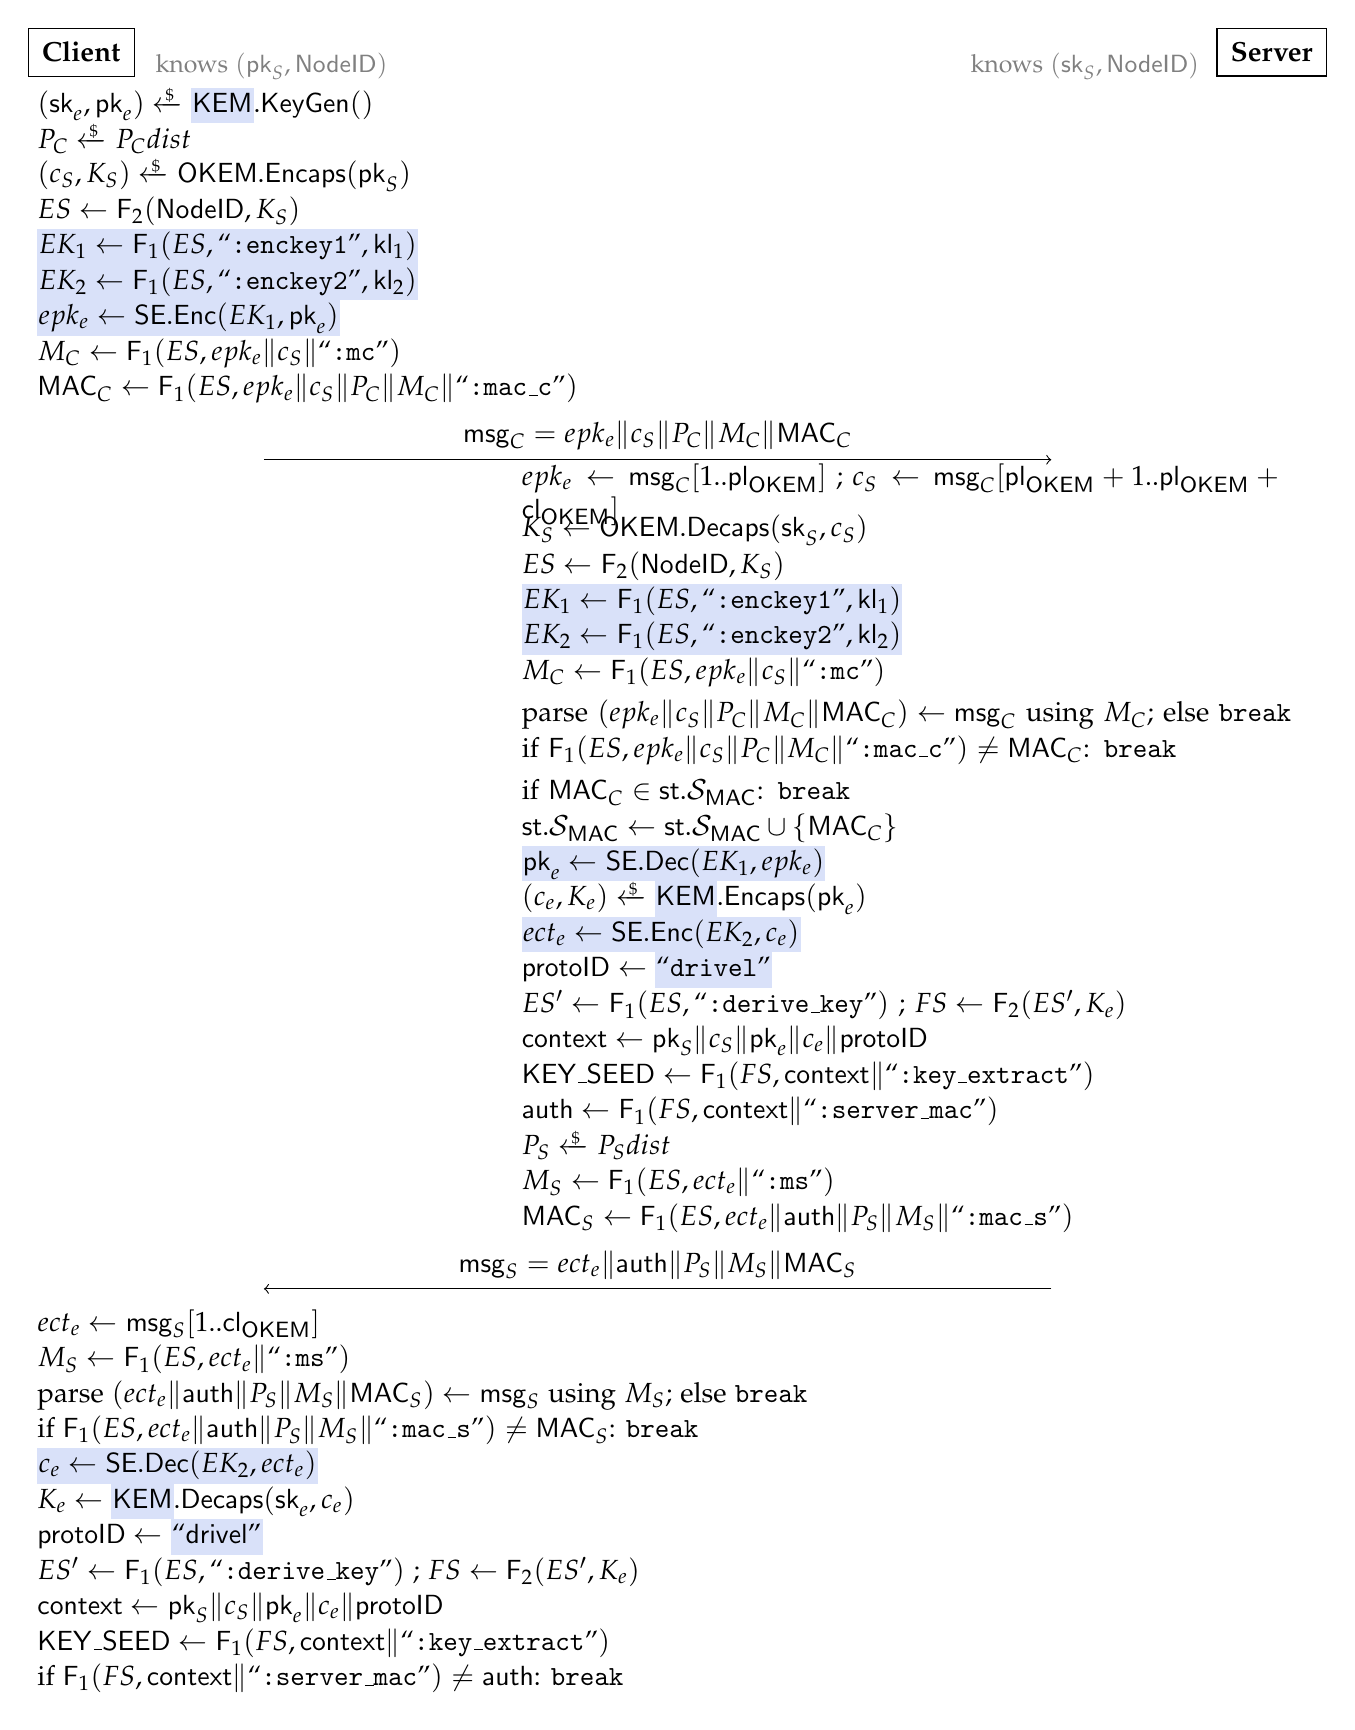
\begin{tikzpicture}
	% Set the X coordinates of the client, server, and arrows
	\edef\ClientX{0}
	%% full page
	\edef\ArrowLeft{3}
	\edef\ArrowRight{13}
	\edef\ServerX{16.5}
	\edef\ServerLeftTextwidth{10.1cm} % width of server-side text, when left-aligned
	%% CCS one column
	% \edef\ArrowLeft{1}
	% \edef\ArrowRight{9}
	% \edef\ServerX{10}
	% \edef\ServerLeftTextwidth{8.25cm} % width of server-side text, when left-aligned
	% Set the starting Y coordinate
	\edef\Y{0}

	% Draw header boxes
	\node [rectangle,draw,inner sep=5pt,right] at (\ClientX,\Y) {\textbf{Client}};
	\node [rectangle,draw,inner sep=5pt,left] at (\ServerX,\Y) {\textbf{Server}};
	
	% \NextLine[0.4]
	% \ClientAction[gray,font=\small]{\hspace{1.25cm}knows $(\pk_S, \nodeid)$}
	% \ServerAction[gray,font=\small]{knows $(\sk_S, \nodeid)$\hspace{1.25cm}\null}
	% \NextLine[1.1]
	
	\NextLine[0.4]
	\ClientAction[gray,font=\small]{\hspace{1.5cm}knows $(\pk_S, \nodeid)$}
	\ServerAction[gray,font=\small]{knows $(\sk_S, \nodeid)$\hspace{1.5cm}\null}
	\NextLine[1.1]
	
	\ClientAction{$(\sk_e, \pk_e) \getsr \highlightbox{\KEM}.\kgen()$} 
	\NextLine
	\ClientAction{$P_C \getsr P_Cdist$}
	\NextLine
	% \ClientAction{\old{$(c_S, K_S) \getsr \KEM.\encaps(\pk_S)$}}
	% \NextLine
	% \ClientAction{\old{$cobf_S \gets \ObfEncode(c_S)$}}
	% \NextLine
	\ClientAction{$(c_S, K_S) \getsr \OKEM.\encaps(\pk_S)$}
	\NextLine
	% \ClientAction{$cobf_S \getsr \OKEM.\ObfCTEnc(c_S)$}
	% \NextLine
	% \ClientAction{\old{$ES \highlightbox{$\conc EK_1 \conc EK_2$} \gets \funComb(\nodeid, K_S)$}}
	% \NextLine
	\ClientAction{$ES \gets \funComb(\nodeid, K_S)$}
	\NextLine
	\ClientAction{\highlightbox{$EK_1 \gets \funPRF(ES, \textlit{:enckey1}, \keylen_1)$}}
	\NextLine
	\ClientAction{\highlightbox{$EK_2 \gets \funPRF(ES, \textlit{:enckey2}, \keylen_2)$}}
	\NextLine
	\ClientAction{\highlightbox{$epk_e \gets \funEnc(EK_1, \pk_e)$}}
	\NextLine
	\ClientAction{$M_C \gets \funPRF(ES, epk_e \conc c_S \conc \textlit{:mc})$}
	%\mar{why do we have this? the previous paper even admits M_C is unnecessary}\mar{because M_S is necessary when the server has content after its response, and this is symmetric}}
	\NextLine
	\ClientAction{$\mathsf{MAC}_C \gets \funPRF(ES, epk_e \conc c_S \conc P_C \conc M_C \conc \textlit{:mac\_c})$}
	
	%%%%%%%%%%%%%%%%%%%%%%%%%%%%%%%%%%%%%%%%%%%%%%%%%%%%%%%%%%%%%%%%%%%%%%%%%%%%%%%%%%%%%%%%%%%%%%%%%%%%%%%
	\NextLine[1.5]
	\ClientToServer{$\mathsf{msg}_C = epk_e \conc c_S \conc P_C \conc M_C \conc \mathsf{MAC}_C$}{}
	\NextLine[1]
	%%%%%%%%%%%%%%%%%%%%%%%%%%%%%%%%%%%%%%%%%%%%%%%%%%%%%%%%%%%%%%%%%%%%%%%%%%%%%%%%%%%%%%%%%%%%%%%%%%%%%%%
	
	\ServerActionLeft{$epk_e \gets \mathsf{msg}_C[1..\obfpklen]$ ; $c_S \gets \mathsf{msg}_C[\obfpklen+1..\obfpklen+\obfctxtlen]$}
	\NextLine
	% \ServerActionLeft{\old{$c_S \gets \ObfDecode(cobf_S)$}}
	% \NextLine
	% \ServerActionLeft{\old{$K_S \gets \KEM.\decaps(\sk_S, c_S)$}}
	% \NextLine
	% \ServerActionLeft{$c_S \gets \OKEM.\ObfCTDec(cobf_S)$}
	% \NextLine
	\ServerActionLeft{$K_S \gets \OKEM.\decaps(\sk_S, c_S)$}
	\NextLine
	% \ServerActionLeft{\old{$ES \highlightbox{$\conc EK_1 \conc EK_2$} \gets \funComb(\nodeid, K_S)$}}
	% \NextLine
	\ServerActionLeft{$ES \gets \funComb(\nodeid, K_S)$}
	\NextLine
	\ServerActionLeft{\highlightbox{$EK_1 \gets \funPRF(ES, \textlit{:enckey1}, \keylen_1)$}}
	\NextLine
	\ServerActionLeft{\highlightbox{$EK_2 \gets \funPRF(ES, \textlit{:enckey2}, \keylen_2)$}}
	\NextLine
	\ServerActionLeft{$M_C \gets \funPRF(ES, epk_e \conc c_S \conc \textlit{:mc})$}
	\NextLine[1.2]
	% \ServerActionLeft{$M_C \gets \HMAC(\cpk^\ltssk, \ltspk \conc \nodeid \conc \ellcpk)$}
	% \NextLine
	\ServerActionLeft{parse $(epk_e \conc c_S \conc P_C \conc M_C \conc \mathsf{MAC}_C) \gets \mathsf{msg}_C$ using $M_C$; else $\texttt{break}$}
	\NextLine
	\ServerActionLeft{if $\funPRF(ES, epk_e \conc c_S \conc P_C \conc M_C \conc \textlit{:mac\_c}) \neq \mathsf{MAC}_C$: $\texttt{break}$}
	\NextLine[1.2]
	\ServerActionLeft{if $\mathsf{MAC}_C \in \pstate.\macregister$: $\texttt{break}$}
	\NextLine
	\ServerActionLeft{$\pstate.\macregister \gets \pstate.\macregister \cup \{\mathsf{MAC}_C\}$}
	\NextLine
	\ServerActionLeft{\highlightbox{$\pk_e \gets \funDec(EK_1, epk_e)$}}
	\NextLine
	% \ServerActionLeft{\old{$(c_e, K_e) \getsr \KEM.\encaps(\pk_e)$}}
	% \NextLine
	% \ServerActionLeft{\old{$cobf_e \gets \ObfEncode(c_e)$}}
	% \NextLine
	\ServerActionLeft{$(c_e, K_e) \getsr \highlightbox{\KEM}.\encaps(\pk_e)$}
	\NextLine
	\ServerActionLeft{\highlightbox{$ect_e \gets \funEnc(EK_2, c_e)$}}
	\NextLine
% 	\ServerActionLeft{$\text{\codecomment{ntor handshake component}}$}
% 	\NextLine
	\ServerActionLeft{$\mathsf{protoID} \gets \highlightbox{\textlit{drivel}}$}
	\NextLine
	\ServerActionLeft{$ES' \gets \funPRF(ES, \textlit{:derive\_key})$ ; $FS \gets \funComb(ES', K_e)$}
	\NextLine
% 	\ServerActionLeft{$FS \gets \funComb(ES', K_e)$}
% 	\NextLine
	\ServerActionLeft{$\mathsf{context} \gets \pk_S \conc c_S \conc \pk_e \conc c_e \conc \mathsf{protoID}$}
	\NextLine
	\ServerActionLeft{$\mathsf{KEY\_SEED} \gets \funPRF(FS, \mathsf{context} \conc \textlit{:key\_extract})$}
	\NextLine
	\ServerActionLeft{$\mathsf{auth} \gets \funPRF(FS, \mathsf{context} \conc \textlit{:server\_mac})$}
	\NextLine
% 	\ServerActionLeft{$\text{\codecomment{end ntor handshake component}}$}
% 	\NextLine
	\ServerActionLeft{$P_S \getsr P_Sdist$} % \text{random bytes of length }[0,8096]$}
	\NextLine
	\ServerActionLeft{$M_S \gets \funPRF(ES, ect_e \conc \textlit{:ms})$}
	\NextLine
	\ServerActionLeft{$\mathsf{MAC}_S \gets \funPRF(ES, ect_e \conc \mathsf{auth} \conc P_S \conc M_S \conc \textlit{:mac\_s})$}
	
	%%%%%%%%%%%%%%%%%%%%%%%%%%%%%%%%%%%%%%%%%%%%%%%%%%%%%%%%%%%%%%%%%%%%%%%%%%%%%%%%%%%%%%%%%%%%%%%%%%%%%%%
	\NextLine[1.5]
	\ServerToClient{$\mathsf{msg}_S = ect_e \conc \mathsf{auth} \conc P_S \conc M_S \conc \mathsf{MAC}_S$}{}
	\NextLine[1]
	%%%%%%%%%%%%%%%%%%%%%%%%%%%%%%%%%%%%%%%%%%%%%%%%%%%%%%%%%%%%%%%%%%%%%%%%%%%%%%%%%%%%%%%%%%%%%%%%%%%%%%%
	
	\ClientAction{$ect_e \gets \mathsf{msg}_S[1..\obfctxtlen]$}
	\NextLine
	\ClientAction{$M_S \gets \funPRF(ES, ect_e \conc \textlit{:ms})$}
	\NextLine
	\ClientAction{parse $(ect_e \conc \mathsf{auth} \conc P_S \conc M_S \conc \mathsf{MAC}_S) \gets \mathsf{msg}_S$ using $M_S$; else $\texttt{break}$}
	\NextLine
	\ClientAction{if $\funPRF(ES, ect_e \conc \mathsf{auth} \conc P_S \conc M_S \conc \textlit{:mac\_s}) \neq \mathsf{MAC}_S$: $\texttt{break}$}
	\NextLine
	% \ClientAction{\old{$c_e \gets \ObfDecode(cobf_e)$}}
	% \NextLine
	% \ClientAction{\old{$K_e \gets \KEM.\decaps(\sk_e, c_e)$}}
	% \NextLine
	\ClientAction{\highlightbox{$c_e \gets \funDec(EK_2, ect_e)$}}
	\NextLine
	\ClientAction{$K_e \gets \highlightbox{\KEM}.\decaps(\sk_e, c_e)$}
	\NextLine
% 	\ClientAction{$\text{\codecomment{ntor handshake component}}$}
% 	\NextLine
	\ClientAction{$\mathsf{protoID} \gets \highlightbox{\textlit{\drivel{}}}$}
	\NextLine
	\ClientAction{$ES' \gets \funPRF(ES, \textlit{:derive\_key})$ ; $FS \gets \funComb(ES', K_e)$}
	\NextLine
% 	\ClientAction{$FS \gets \funComb(ES', K_e)$}
% 	\NextLine
	\ClientAction{$\mathsf{context} \gets \pk_S \conc c_S \conc \pk_e \conc c_e \conc \mathsf{protoID}$}
	\NextLine
	\ClientAction{$\mathsf{KEY\_SEED} \gets \funPRF(FS, \mathsf{context} \| \textlit{:key\_extract}) $}
	\NextLine
	\ClientAction{if $\funPRF(FS, \mathsf{context} \conc \textlit{:server\_mac}) \neq \mathsf{auth}$: $\texttt{break}$}
\end{tikzpicture}
}

    \caption[
        The modified drivel TODO.
    ]{
        The Drivel obfuscated key exchange protocol TODO.
        OKEM is an OKEM satisfying IND-CCA, SPR-CCA, and ciphertext uniformity.
        KEM is an IND-1CCA-secure KEM.
        SE is an OT-IND-secure symmetric encryption scheme.
        F1 is a PRF and F2 is a dual PRF.
        Core differences to the pq-obfs protocol from [GSV24] are highlighted in blue boxes.
    }
    \label{fig:modified-drivel}
\end{figure}

\section{Implementation} \label{sec:implementation}

* (Experimenting with implementing different traffic patterns, such as arbitrary fragmentation of key
exchange messages and/or more flexibility in clients to send arbitrary data)


=> For Tor people: Consider as part of audience of report, so also accessible to non-crypto-nerds and illustrate: How to deploy, How to use, Integration barriers such as SOCKS issues -> Implementation section

\chapter{Experimental Evaluation}\label{ch:results}

\section{Experiment Setup} \label{sec:experiment-setup}

* performance and traffic overhead compared to the original obfs4 protocol
* (efficacy of the protocol against blocking in censored regions)

\section{Measurement Results} \label{sec:measurement-results}

\section{Conclusions} \label{sec:conclusion}


% \appendix
% \input{sections/6_appendix}

\backmatter

\bibliographystyle{plain}
\bibliography{cryptobib/abbrev3,cryptobib/crypto,refs}

%\includepdf[pages={-}]{declaration-originality-signed.pdf}

\end{document}
